\documentclass[cn, 11pt, fancy, hide]{elegantbook}

\usepackage{natbib}
\bibliographystyle{apalike}

\hypersetup{
  pdfcreator={LaTeX via pandoc}}


\usepackage{longtable,booktabs}



\setlength{\emergencystretch}{3em}  % prevent overfull lines
\providecommand{\tightlist}{%
  \setlength{\itemsep}{0pt}\setlength{\parskip}{0pt}}

\setcounter{secnumdepth}{5}

%%% Use protect on footnotes to avoid problems with footnotes in titles
\let\rmarkdownfootnote\footnote%
\def\footnote{\protect\rmarkdownfootnote}

  \title{从统计到预测:数据科学背景下精准科研信息服务}

\subtitle{2020年个人版}

  \author{王敏杰}

  \date{2020-06-21}

% logo 图案
  \logo{figure/logo.png}
% 封面图片
  \cover{figure/cover.jpg}
% 版本号
  \version{0.1}
% 机构名
% 引用格言
  \extrainfo{Victory won't come to us unless we go to it. --- M. Moore}
% 导言区 preamble
\usepackage{framed,color}
\definecolor{shadecolor}{RGB}{248,248,248}

\frontmatter
\usepackage{booktabs}
\usepackage{longtable}
\usepackage{array}
\usepackage{multirow}
\usepackage{wrapfig}
\usepackage{float}
\usepackage{colortbl}
\usepackage{pdflscape}
\usepackage{tabu}
\usepackage{threeparttable}
\usepackage{threeparttablex}
\usepackage[normalem]{ulem}
\usepackage{makecell}
\usepackage{xcolor}

\begin{document}
% 封面
\maketitle
% 插入 before_body.tex

% 目录
{
\setcounter{tocdepth}{2}
\tableofcontents
}
% 表目录
% 图目录
% 书籍主体部分
\mainmatter

\hypersetup{pageanchor=true}

\hypertarget{ux524dux8a00}{%
\chapter*{前言}\label{ux524dux8a00}}
\addcontentsline{toc}{chapter}{前言}

根据基本科学指标数据库(Essential Science Indicators,简称ESI)发布的最新统计数据显示:

1、我国师范类院校有 ESI 学科的 25 所,北京师范大学进入 ESI 学科数量最多。从
入选的学科来看,其中化学学科的频次最高。

2、我校工程学近十年累积被引频次2781,距离ESI前1\%学科阈值线2755, 接近度106\%,有望入选ESI学科,但竞争依然激烈。

3、根据贝叶斯数学模型分析,我校工程学科2020年有约80\%的概率进入ESI前百分之一学科。

4、西华师范大学工程学(被引频次2922)和西华大学工程学(被引频次2808)先后进入了ESI前百分之一学科。

\hypertarget{ux6570ux636eux6765ux6e90}{%
\section*{数据来源}\label{ux6570ux636eux6765ux6e90}}
\addcontentsline{toc}{section}{数据来源}

Essential Science Indicator(基本科学指标,以下简称ESI)是由世界上著名的学术信息出版机构美国科技信息所(ISI)于2001年推出的一种文献评价分析工具,是基于SCI和SSCI所收录的全球11000多种学术期刊的1000多万条文献记录而建立的计量分析数据库。

\hypertarget{ux7edfux8ba1ux53e3ux5f84}{%
\section*{统计口径}\label{ux7edfux8ba1ux53e3ux5f84}}
\addcontentsline{toc}{section}{统计口径}

\begin{itemize}
\tightlist
\item
  统计对象:师范类大学
\item
  技术指标:由ESI说了算
\item
  统计周期:与当前ESI阈值计算所覆盖的时间一致(比如:2010年全年 - 2020年)
\item
  命名规则:与检索词一致。不同的数据库来源,分别用不同的文件夹保存
\end{itemize}

\begin{verbatim}
#>  [1] "Anhui Normal University.csv"         "Beijing Normal University.csv"      
#>  [3] "Capital Normal University.csv"       "Central China Normal University.csv"
#>  [5] "Chongqing Normal University.csv"     "East China Normal University.csv"   
#>  [7] "Fujian Normal University.csv"        "Guangxi Normal University.csv"      
#>  [9] "Guizhou Normal University.csv"       "Hainan Normal University.csv"       
#> [11] "Hangzhou Normal University.csv"      "Harbin Normal University.csv"       
#> [13] "Hebei Normal University.csv"         "Henan Normal University.csv"        
#> [15] "Hunan Normal University.csv"         "Jiangsu Normal University.csv"      
#> [17] "Jiangxi Normal University.csv"       "Liaoning Normal University.csv"     
#> [19] "Nanjing Normal University.csv"       "Northeast Normal University.csv"    
#> [21] "Northwest Normal University.csv"     "Qufu Normal University.csv"         
#> [23] "Shaanxi Normal University.csv"       "Shandong Normal University.csv"     
#> [25] "Shanghai Normal University.csv"      "Sichuan Normal University.csv"      
#> [27] "South China Normal University.csv"   "Tianjin Normal University.csv"      
#> [29] "Yunnan Normal University.csv"        "Zhejiang Normal University.csv"
\end{verbatim}

\hypertarget{ux6280ux672fux6307ux6807}{%
\section*{技术指标}\label{ux6280ux672fux6307ux6807}}
\addcontentsline{toc}{section}{技术指标}

\begin{itemize}
\tightlist
\item
  什么是ESI学科分类
\end{itemize}

ESI数据库将收录期刊划分为22个学科,再按学科进行各项统计。每种期刊只会分入一个学科,只有被归类为跨学科学科(MULTIDISCIPLINARY)的Science、Nature与PNAS期刊,会被按照各篇文章的参考文献与引用文献,重新为每篇文章单独分类,但每篇文章仍只会被分类到一个学科。

\begin{itemize}
\tightlist
\item
  什么叫进入ESI前百分之一学科
\end{itemize}

ESI数据库以引文分析为基础,以10年为1个周期对全球所有大学及科研机构的SCI、SSCI论文的被引频次按22个学科进行由高到低排序,被引频次排在前1\%的学科,称为该机构进入ESI前1\%学科。

\begin{itemize}
\tightlist
\item
  ESI学科阈值(ESI Thresholds)
\end{itemize}

近十年,某一ESI学科被引次数排在前1\%的作者和机构的最低被引次数。

\begin{itemize}
\tightlist
\item
  被引频次已经超过阈值线,但为什么没有进入ESI前百分之一学科
\end{itemize}

主要有两方面的原因:一是统计来源不同,本报告的数据来源于INCITES、ESI、WoS数据库,INCITES、WoS用于查找机构学科论文的被引频次、论文数量等数据,ESI用于查看ESI学科基准线、学科阈值等数据,三个库存在数据更新不同步的现象,故在INCITES、WoS数据库中查到的被引频次,高于ESI数据库中的被引频次;二是INCITES、WoS数据库查到的被引频次包含会议文献的被引频次,而ESI只统计论文和综述两种文献的被引频次,因此得到的被引频次会有虚高现象。

\begin{itemize}
\tightlist
\item
  高被引论文和热点论文
\end{itemize}

指同一年同一个ESI学科发表论文的被引次数按由高到低进行排序,排在前1\%的论文;热点论文统计某一ESI学科最近两年发表的论文,按照最近两个月被引用次数进入前0.1\%的论文而给出。
高被引论文和热点论文有助于确定一个研究领域内的突破性研究,并在科学网络中用于确定和提炼最有影响力的研究论文;同时高被引论文的数量在很大程度上决定学科能否进入前1\%。

\begin{itemize}
\tightlist
\item
  高被引论文与进入ESI前百分之一学科的关系
\end{itemize}

高被引论文越多,进入ESI前百分之一学科的概率越大。

\hypertarget{ux8fdbux5ea6ux8868}{%
\section*{进度表}\label{ux8fdbux5ea6ux8868}}
\addcontentsline{toc}{section}{进度表}

\begin{itemize}
\tightlist
\item
  文献调研(3月底完成)
\item
  数据获取(4月中旬完成)
\item
  数学分析和模型评估(5月初完成)
\item
  报告初稿(5月中旬完成)
\item
  研讨会(待定)
\item
  正式稿发布(待定)
\end{itemize}

\hypertarget{ux5173ux4e8eux672cux6587ux6863}{%
\section*{关于本文档}\label{ux5173ux4e8eux672cux6587ux6863}}
\addcontentsline{toc}{section}{关于本文档}

本报告使用R和Stan语言完成,严重依赖\texttt{tidyverse}和\texttt{tidyESI}宏包,数据和代码存放在GitHub仓库\url{https://github.com/perlatex/use_tidyESI},欢迎批评指正。

\hypertarget{ux611fux8c22}{%
\section*{感谢}\label{ux611fux8c22}}
\addcontentsline{toc}{section}{感谢}

I am very grateful to \href{https://github.com/bbbales2}{Ben Bales} from the Stan Development Team for his patience in guiding Stan code.
感谢彭凤老师在图书购买上提供的帮助,感谢研究生李晨阳协助完成数据收集和整理工作。感谢科睿唯安 (原汤森路透) 公司赵宇先生提供了非常专业地技术解释。

\hypertarget{author}{%
\chapter*{关于作者}\label{author}}
\addcontentsline{toc}{chapter}{关于作者}

王敏杰,四川师范大学研究生公选课《数据科学中的R语言》和《社会科学中的统计学》授课老师,毕业于西南交通大学量子物理专业,爱好数据科学,喜欢用R和Stan统计编程,
联系方式 \href{mailto:38552109@qq.com}{\nolinkurl{38552109@qq.com}}

\hypertarget{bigdata}{%
\chapter{师范院校}\label{bigdata}}

为增强中国高校的综合实力和学科竞争力,2015年11月,国务院印发《统筹推进世界一流大学和一流学科建设总体方案》,对我国高校迈进世界一流大学和一流学科行列的数量与质量提出了要求,明确指出要通过一流学科的建设带动世界一流大学的建设。在此背景下,北京、上海、广东、浙江等省市相继出台了各自的一流学科建设方案。2017年1月,教育部、
财政部和国家发展改革委联合印发了《统筹推进世界一流大学和一流学科建设实施办法(暂行)》,特别强调要以学科为基础,充分利用有影响力的第三方评价,强化学科建设绩效考核,为学科的发展建设提供有效参考。

ESI(Essential Science Indicators,基本科学指标数据库)是2001年美国科技信息所(ISI)推出的衡量科学研究绩效、跟踪科学发展趋势的分析评价工具,具有数据权威可量化、国际可比较、能够实现对学科建设绩效的动态监测等优点,是当今国际公认的评价高校学科发展水平和影响力的重要工具之一。基于ESI的科研竞争力评估得到国内各级教育主管部门和各大高校的认可和重视,已成为衡量高校学科发展和学术影响力的共性指标,如在申报``面向科学前沿的协同创
新中心''、第四轮学科评估及遴选重点支持高校等项目中,均把ESI学科数、高被引论文数作为重要指标。

本文利用2020年05月14日科睿唯安发布的新一期ESI数据进行统计调查,数据覆盖时间为2010年1月至2020年02月,以定量分析的方法展现中国大陆师范类高校(Top30)在ESI学科的发展现状和趋势。

横向对比发现, 四川师范大学经过多年努力,学科竞争力稳步提升,学科建设取得了一定成效,学术水平显著提高。ESI论文数和总被引频次整体呈上升的趋势, 但学科影响力相对较弱,ESI前百分之一学科至今还未实现零的突破。

\hypertarget{ux79d1ux7814ux4ea7ux51fa}{%
\section{科研产出}\label{ux79d1ux7814ux4ea7ux51fa}}

\begin{table}[!h]

\caption{\label{tab:unnamed-chunk-4}师范院校发展情况}
\centering
\begin{tabular}[t]{lrr}
\toprule
univ\_cn & n\_paper & n\_cited\\
\midrule
安徽师范大学 & 5309 & 79687\\
北京师范大学 & 33283 & 511749\\
首都师范大学 & 8167 & 92554\\
华中师范大学 & 12420 & 242724\\
重庆师范大学 & 2942 & 28601\\
\addlinespace
华东师范大学 & 23870 & 361202\\
福建师范大学 & 6602 & 69344\\
广西师范大学 & 4965 & 58162\\
贵州师范大学 & 1777 & 13193\\
海南师范大学 & 1603 & 13211\\
\bottomrule
\end{tabular}
\end{table}

画出来看看

\begin{center}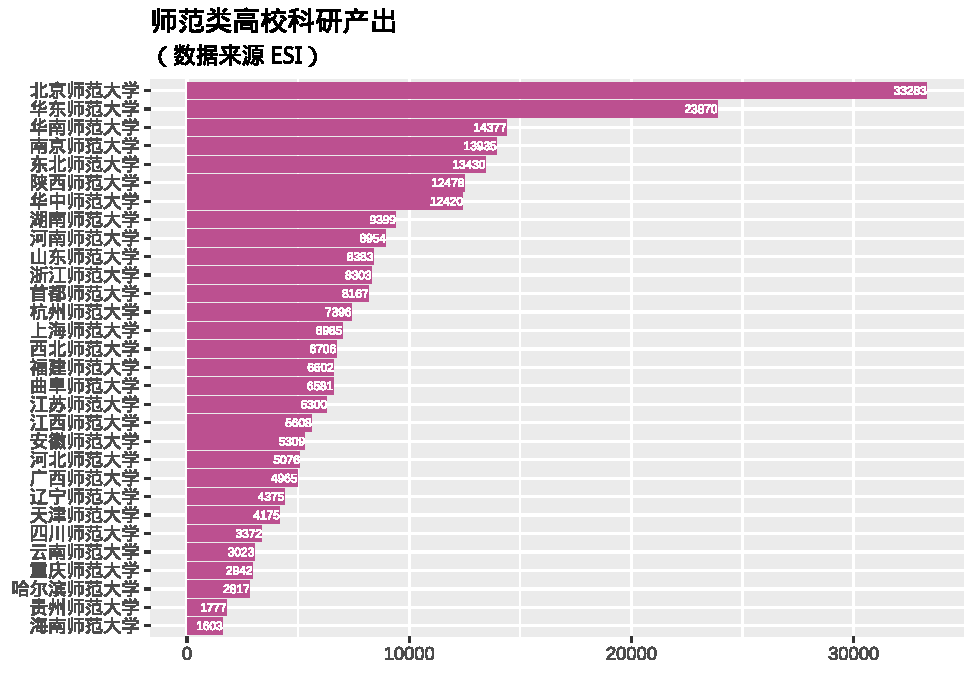
\includegraphics[width=1\linewidth]{ElegantBookdown_files/figure-latex/unnamed-chunk-5-1} \end{center}

\hypertarget{ux5b66ux79d1ux53d1ux5c55}{%
\section{学科发展}\label{ux5b66ux79d1ux53d1ux5c55}}

\begin{table}[!h]

\caption{\label{tab:unnamed-chunk-6}师范大学学科发展}
\centering
\begin{tabular}[t]{lll}
\toprule
univ\_cn & discipline\_cn & year\_range\\
\midrule
安徽师范大学 & 化学 & 2010\\
安徽师范大学 & 化学 & 2011\\
安徽师范大学 & 化学 & 2012\\
安徽师范大学 & 化学 & 2013\\
安徽师范大学 & 化学 & 2014\\
\bottomrule
\end{tabular}
\end{table}

\begin{center}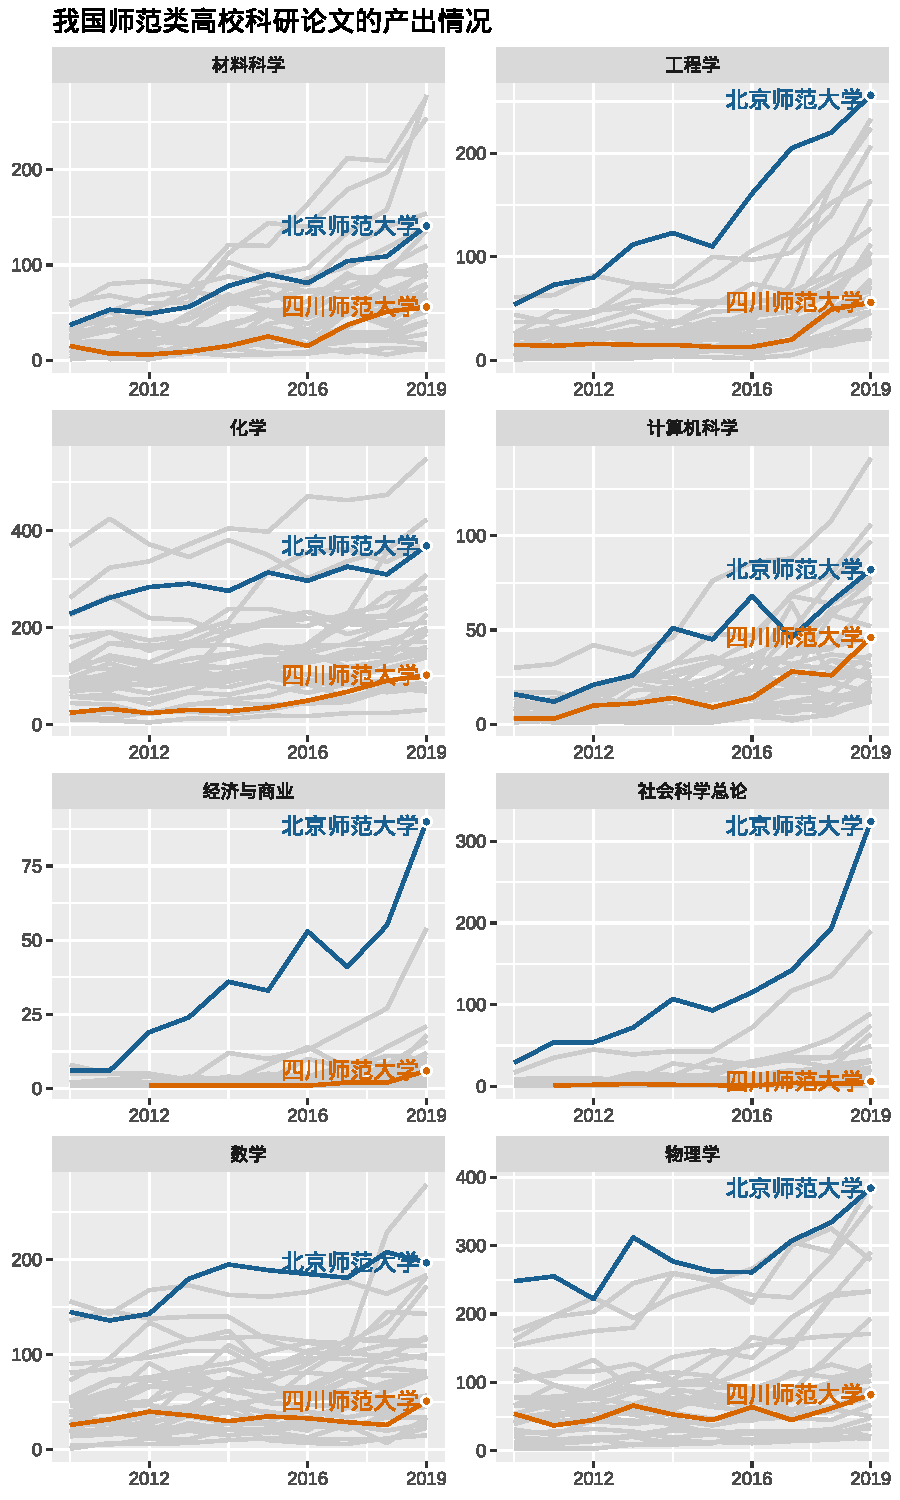
\includegraphics[width=1\linewidth]{ElegantBookdown_files/figure-latex/unnamed-chunk-9-1} \end{center}

这里我们高亮了\textbf{北京师范大学}和\textbf{四川师范大学}两所高校的发展曲线, 灰色背景的其他28所高校的发展情况。可见,近几年我国师范类高校科研论文的产出整体上稳步提升,
符合科学发展规律。但也明显看到,四川师范大学作为西部高校,与东部发达地区的院校还存在一定的距离。

\hypertarget{ux5e08ux8303ux7c7bux9662ux6821ux8fdbux5165ux524dux767eux5206ux4e4bux4e00esiux5b66ux79d1ux7684ux6570ux91cf}{%
\section{师范类院校进入前百分之一ESI学科的数量}\label{ux5e08ux8303ux7c7bux9662ux6821ux8fdbux5165ux524dux767eux5206ux4e4bux4e00esiux5b66ux79d1ux7684ux6570ux91cf}}

这里我们整理了师范类院校进入前百分之一ESI学科的数量。从学校来看,师范类院校有ESI学科的25所,其中最多的是北京师范大学14个学科,华东师范大学12个学科, 南京师范大学8个学科。从入选的学科来看,化学学科、材料学科和工程学入选频次最高。

\begin{verbatim}
#> Please make sure the source information is up to date.
\end{verbatim}

\begin{center}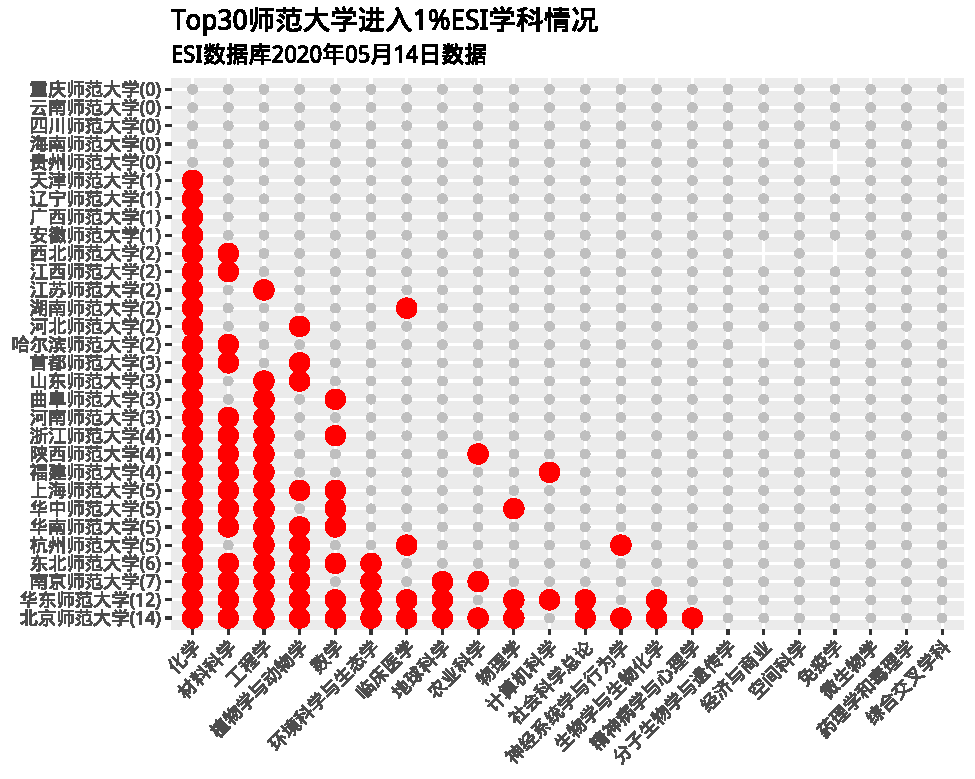
\includegraphics[width=1\linewidth]{ElegantBookdown_files/figure-latex/unnamed-chunk-11-1} \end{center}

\hypertarget{ux5e08ux8303ux9662ux6821ux5404ux5b66ux79d1ux53d1ux5c55ux6001ux52bf}{%
\section{师范院校各学科发展态势}\label{ux5e08ux8303ux9662ux6821ux5404ux5b66ux79d1ux53d1ux5c55ux6001ux52bf}}

为跟踪学科发展态势,这里我们考察了各师范类高校在两个维度(累计产出和累计影响力)上的科研表现情况,图中红色标注表示该校已经进入前百分之一ESI学科,灰色表示还没有进入前百分之一ESI学科,由于ESI数据库比SCI数据库滞后两个月,因此图中阈值线附近的点,会有细微的偏差(可以理解为图中的阈值线会有细微的偏差)。

\begin{verbatim}
#> Please make sure the source information is up to date.
\end{verbatim}

\hypertarget{ux5de5ux7a0bux5b66}{%
\subsection{工程学}\label{ux5de5ux7a0bux5b66}}

\begin{center}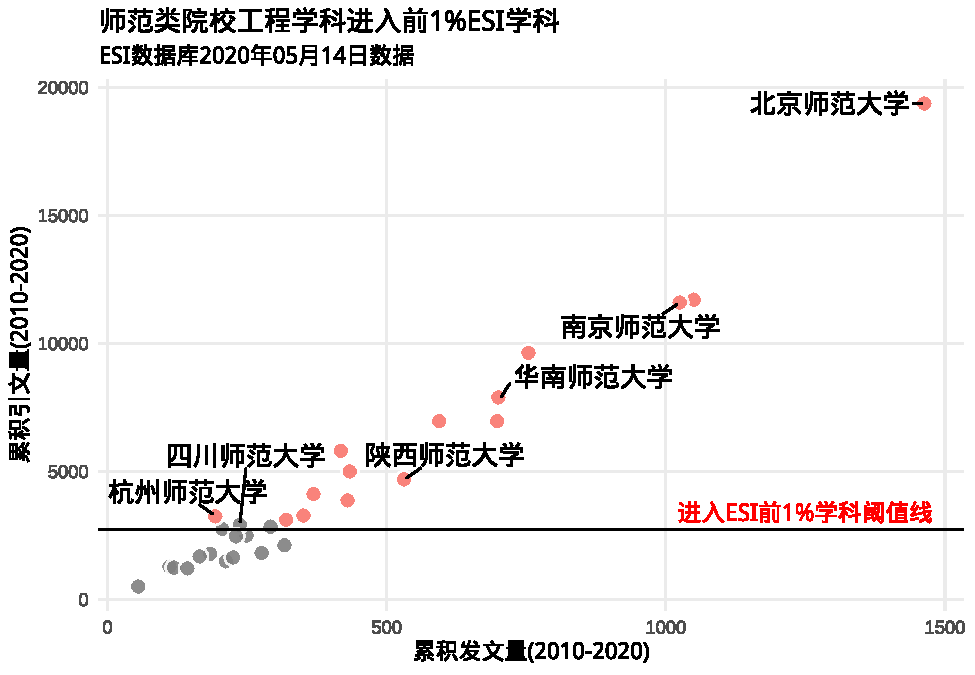
\includegraphics[width=1\linewidth]{ElegantBookdown_files/figure-latex/unnamed-chunk-13-1} \end{center}

四川师范大学的科研产出超过杭州师范大学,但科研影响力差一点点,因此杭州师范大学率先进入了前百分之一ESI学科。

\hypertarget{ux5316ux5b66}{%
\subsection{化学}\label{ux5316ux5b66}}

\begin{center}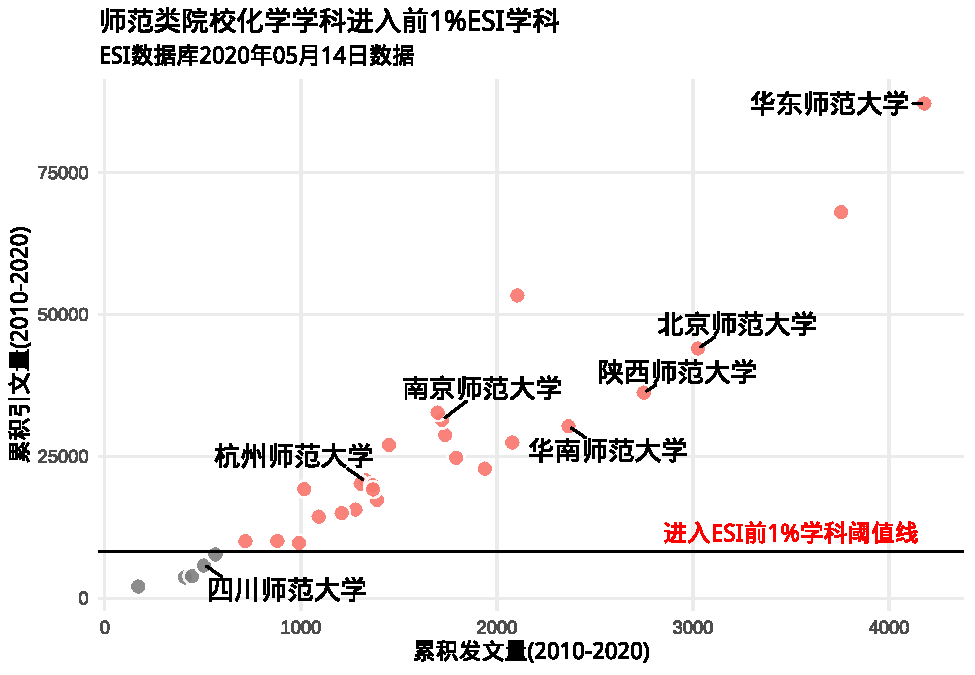
\includegraphics[width=1\linewidth]{ElegantBookdown_files/figure-latex/unnamed-chunk-14-1} \end{center}

\hypertarget{ux7269ux7406ux5b66}{%
\subsection{物理学}\label{ux7269ux7406ux5b66}}

\begin{center}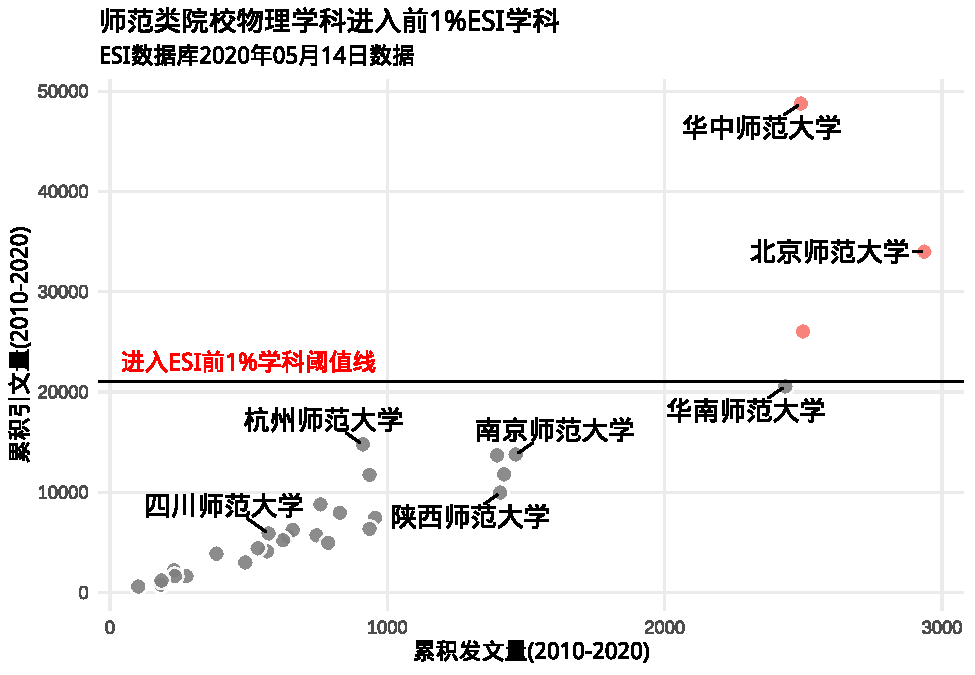
\includegraphics[width=1\linewidth]{ElegantBookdown_files/figure-latex/unnamed-chunk-15-1} \end{center}

\hypertarget{ux6570ux5b66}{%
\subsection{数学}\label{ux6570ux5b66}}

\begin{center}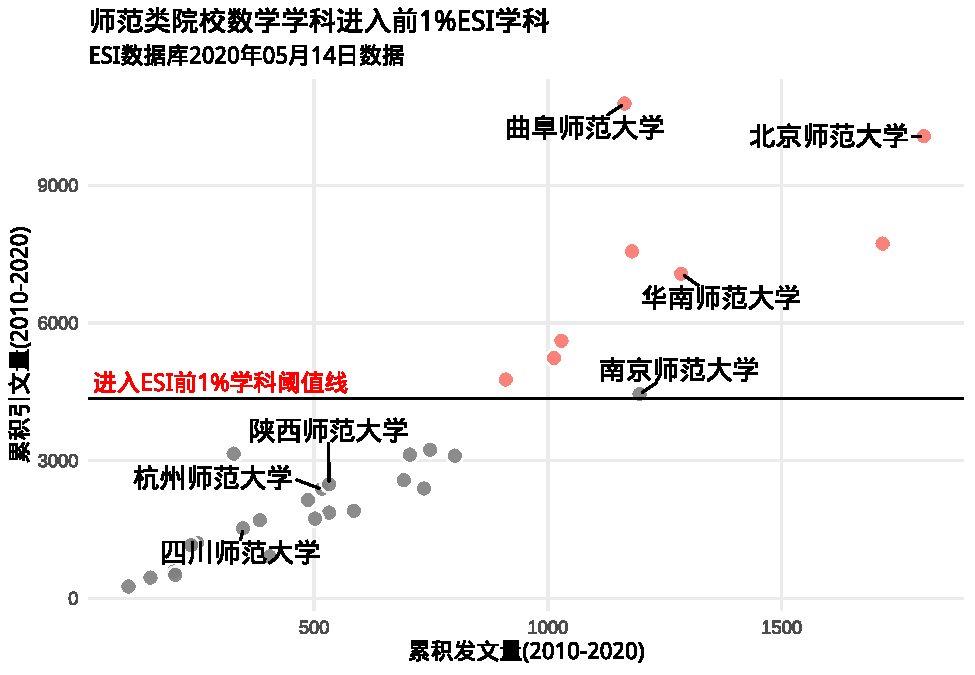
\includegraphics[width=1\linewidth]{ElegantBookdown_files/figure-latex/unnamed-chunk-16-1} \end{center}

\hypertarget{progress}{%
\chapter{学科发展}\label{progress}}

\hypertarget{ux6f5cux529bux5b66ux79d1}{%
\section{潜力学科}\label{ux6f5cux529bux5b66ux79d1}}

当前四川师范大学在励精图治奋力耕耘,推动学科发展,其中\textbf{工程学}学科与进入ESI学科的阈值线最为接近,接近程度达到97.8\%。其他各学科的发展情况见表 \ref{tab:iris} 。

\begin{verbatim}
#> Please make sure the source information is up to date.
\end{verbatim}

\begin{table}[!h]

\caption{\label{tab:iris}四川师范大学进入22ESI学科接近程度}
\centering
\begin{tabular}[t]{lrrrl}
\toprule
学科 & 累积论文数 & 被引频次 & 阈值线 & 接近程度\\
\midrule
工程学 & 237 & 2923 & 2755 & 106.10\%\\
化学 & 505 & 5752 & 8188 & 70.25\%\\
计算机科学 & 167 & 2473 & 3686 & 67.09\%\\
材料科学 & 243 & 2811 & 6674 & 42.12\%\\
数学 & 348 & 1526 & 4359 & 35.01\%\\
\addlinespace
物理学 & 572 & 5893 & 21050 & 28.00\%\\
环境科学与生态学 & 94 & 536 & 4388 & 12.22\%\\
植物学与动物学 & 54 & 336 & 2881 & 11.66\%\\
精神病学与心理学 & 50 & 364 & 4077 & 8.93\%\\
社会科学总论 & 25 & 107 & 1530 & 6.99\%\\
\addlinespace
经济与商业 & 15 & 241 & 4516 & 5.34\%\\
农业科学 & 35 & 85 & 2361 & 3.60\%\\
临床医学 & 16 & 99 & 3374 & 2.93\%\\
神经系统学与行为学 & 14 & 150 & 6426 & 2.33\%\\
微生物学 & 19 & 100 & 5492 & 1.82\%\\
\addlinespace
地球科学 & 22 & 104 & 6140 & 1.69\%\\
药理学和毒理学 & 18 & 53 & 3453 & 1.53\%\\
分子生物学与遗传学 & 40 & 215 & 14132 & 1.52\%\\
生物学与生物化学 & 35 & 93 & 6316 & 1.47\%\\
空间科学 & 2 & 152 & 40196 & 0.38\%\\
\addlinespace
综合交叉学科 & 1 & 2 & 2608 & 0.08\%\\
免疫学 & 1 & 0 & 5149 & 0.00\%\\
\bottomrule
\end{tabular}
\end{table}

\hypertarget{ux7adeux4e89ux5bf9ux624b}{%
\section{竞争对手}\label{ux7adeux4e89ux5bf9ux624b}}

由表 \ref{tab:iris}可以看出\textbf{工程学}是入选前百分之一ESI学科的 潜力学科,但我们也要意识到,当前师范院校高校中,工程学进入ESI学科的有14所,未进入的16所,表 \ref{tab:iris3}列出了这未进入的16所高校的工程学科与阈值线的接近程度,可以看到,大学彼此之间竞争还很激烈。

\begin{table}[!h]

\caption{\label{tab:iris2}工程学科有可能进入ESI学科的师范大学}
\centering
\begin{tabular}[t]{lrrrl}
\toprule
学校 & 累积论文数 & 累积被引频次 & 阈值线 & 接近程度\\
\midrule
四川师范大学 & 237 & 2923 & 2755 & 106.10\%\\
重庆师范大学 & 292 & 2850 & 2755 & 103.45\%\\
广西师范大学 & 206 & 2755 & 2755 & 100.00\%\\
西北师范大学 & 249 & 2500 & 2755 & 90.74\%\\
云南师范大学 & 230 & 2474 & 2755 & 89.80\%\\
\addlinespace
湖南师范大学 & 317 & 2129 & 2755 & 77.28\%\\
首都师范大学 & 276 & 1823 & 2755 & 66.17\%\\
江西师范大学 & 184 & 1791 & 2755 & 65.01\%\\
辽宁师范大学 & 165 & 1690 & 2755 & 61.34\%\\
天津师范大学 & 225 & 1650 & 2755 & 59.89\%\\
\addlinespace
安徽师范大学 & 212 & 1501 & 2755 & 54.48\%\\
贵州师范大学 & 111 & 1288 & 2755 & 46.75\%\\
哈尔滨师范大学 & 119 & 1253 & 2755 & 45.48\%\\
河北师范大学 & 143 & 1223 & 2755 & 44.39\%\\
海南师范大学 & 55 & 515 & 2755 & 18.69\%\\
\bottomrule
\end{tabular}
\end{table}

\begin{table}[!h]

\caption{\label{tab:iris3}师范类院校的工程学科进入ESI前百分之一学科的情况}
\centering
\begin{tabular}[t]{lrrrll}
\toprule
学校 & 累积论文数 & 累积被引频次 & 阈值线 & 接近程度 & 进入ESI\\
\midrule
北京师范大学 & 1463 & 19377 & 2755 & 703.34\% & 是\\
华东师范大学 & 1050 & 11714 & 2755 & 425.19\% & 是\\
南京师范大学 & 1025 & 11602 & 2755 & 421.13\% & 是\\
曲阜师范大学 & 754 & 9640 & 2755 & 349.91\% & 是\\
华南师范大学 & 700 & 7900 & 2755 & 286.75\% & 是\\
\addlinespace
浙江师范大学 & 594 & 6974 & 2755 & 253.14\% & 是\\
山东师范大学 & 698 & 6972 & 2755 & 253.07\% & 是\\
东北师范大学 & 418 & 5815 & 2755 & 211.07\% & 是\\
江苏师范大学 & 434 & 5008 & 2755 & 181.78\% & 是\\
陕西师范大学 & 531 & 4698 & 2755 & 170.53\% & 是\\
\addlinespace
福建师范大学 & 369 & 4124 & 2755 & 149.69\% & 是\\
河南师范大学 & 430 & 3878 & 2755 & 140.76\% & 是\\
上海师范大学 & 351 & 3285 & 2755 & 119.24\% & 是\\
杭州师范大学 & 193 & 3255 & 2755 & 118.15\% & 是\\
华中师范大学 & 320 & 3121 & 2755 & 113.28\% & 是\\
\addlinespace
四川师范大学 & 237 & 2923 & 2755 & 106.10\% & 否\\
重庆师范大学 & 292 & 2850 & 2755 & 103.45\% & 否\\
广西师范大学 & 206 & 2755 & 2755 & 100.00\% & 否\\
西北师范大学 & 249 & 2500 & 2755 & 90.74\% & 否\\
云南师范大学 & 230 & 2474 & 2755 & 89.80\% & 否\\
\addlinespace
湖南师范大学 & 317 & 2129 & 2755 & 77.28\% & 否\\
首都师范大学 & 276 & 1823 & 2755 & 66.17\% & 否\\
江西师范大学 & 184 & 1791 & 2755 & 65.01\% & 否\\
辽宁师范大学 & 165 & 1690 & 2755 & 61.34\% & 否\\
天津师范大学 & 225 & 1650 & 2755 & 59.89\% & 否\\
\addlinespace
安徽师范大学 & 212 & 1501 & 2755 & 54.48\% & 否\\
贵州师范大学 & 111 & 1288 & 2755 & 46.75\% & 否\\
哈尔滨师范大学 & 119 & 1253 & 2755 & 45.48\% & 否\\
河北师范大学 & 143 & 1223 & 2755 & 44.39\% & 否\\
海南师范大学 & 55 & 515 & 2755 & 18.69\% & 否\\
\bottomrule
\end{tabular}
\end{table}

\hypertarget{ux6709ux6548ux8bbaux6587ux6570}{%
\section{有效论文数}\label{ux6709ux6548ux8bbaux6587ux6570}}

这里需要使用
\texttt{tidyESI::add\_is\_enter\_top(univ,\ discipline,\ source\ =\ enter,\ .keep\ =\ TRUE)}获得有效论文数和有效被引频次. 我认为这是很有价值的一张表

\begin{verbatim}
#> Please make sure the source information is up to date.
\end{verbatim}

\begin{table}[!h]

\caption{\label{tab:unnamed-chunk-20}师范类院校的工程学科进入ESI前百分之一学科的情况}
\centering
\begin{tabular}[t]{lrrrrrll}
\toprule
学校 & 累积论文数 & 累积被引频次 & 有效论文数 & 有效被引频次 & 阈值线 & 接近程度 & 进入ESI\\
\midrule
北京师范大学 & 1463 & 19377 & 1408 & 17751 & 2755 & 703.34\% & 是\\
华东师范大学 & 1050 & 11714 & 1014 & 10104 & 2755 & 425.19\% & 是\\
南京师范大学 & 1025 & 11602 & 998 & 10055 & 2755 & 421.13\% & 是\\
曲阜师范大学 & 754 & 9640 & 739 & 8403 & 2755 & 349.91\% & 是\\
华南师范大学 & 700 & 7900 & 683 & 7241 & 2755 & 286.75\% & 是\\
\addlinespace
浙江师范大学 & 594 & 6974 & 584 & 6285 & 2755 & 253.14\% & 是\\
山东师范大学 & 698 & 6972 & 677 & 6418 & 2755 & 253.07\% & 是\\
东北师范大学 & 418 & 5815 & 405 & 5201 & 2755 & 211.07\% & 是\\
江苏师范大学 & 434 & 5008 & 428 & 4419 & 2755 & 181.78\% & 是\\
陕西师范大学 & 531 & 4698 & 521 & 4195 & 2755 & 170.53\% & 是\\
\addlinespace
福建师范大学 & 369 & 4124 & 362 & 3798 & 2755 & 149.69\% & 是\\
河南师范大学 & 430 & 3878 & 418 & 3633 & 2755 & 140.76\% & 是\\
上海师范大学 & 351 & 3285 & 343 & 3008 & 2755 & 119.24\% & 是\\
杭州师范大学 & 193 & 3255 & 190 & 2939 & 2755 & 118.15\% & 是\\
华中师范大学 & 320 & 3121 & 312 & 2765 & 2755 & 113.28\% & 是\\
\addlinespace
四川师范大学 & 237 & 2923 &  &  & 2755 & 106.10\% & 否\\
重庆师范大学 & 292 & 2850 &  &  & 2755 & 103.45\% & 否\\
广西师范大学 & 206 & 2755 &  &  & 2755 & 100.00\% & 否\\
西北师范大学 & 249 & 2500 &  &  & 2755 & 90.74\% & 否\\
云南师范大学 & 230 & 2474 &  &  & 2755 & 89.80\% & 否\\
\addlinespace
湖南师范大学 & 317 & 2129 &  &  & 2755 & 77.28\% & 否\\
首都师范大学 & 276 & 1823 &  &  & 2755 & 66.17\% & 否\\
江西师范大学 & 184 & 1791 &  &  & 2755 & 65.01\% & 否\\
辽宁师范大学 & 165 & 1690 &  &  & 2755 & 61.34\% & 否\\
天津师范大学 & 225 & 1650 &  &  & 2755 & 59.89\% & 否\\
\addlinespace
安徽师范大学 & 212 & 1501 &  &  & 2755 & 54.48\% & 否\\
贵州师范大学 & 111 & 1288 &  &  & 2755 & 46.75\% & 否\\
哈尔滨师范大学 & 119 & 1253 &  &  & 2755 & 45.48\% & 否\\
河北师范大学 & 143 & 1223 &  &  & 2755 & 44.39\% & 否\\
海南师范大学 & 55 & 515 &  &  & 2755 & 18.69\% & 否\\
\bottomrule
\end{tabular}
\end{table}

\hypertarget{ux597dux770bux7684ux8868ux683cux683c}{%
\section{好看的表格格}\label{ux597dux770bux7684ux8868ux683cux683c}}

\begin{table}[!h]

\caption{\label{tab:unnamed-chunk-21}师范类院校的工程学科进入ESI前百分之一学科的情况}
\centering
\begin{tabular}[t]{lrrrrrll}
\toprule
学校 & \makecell[c]{累积 \\ 论文数} & \makecell[c]{累积 \\ 被引频次} & \makecell[c]{有效 \\ 论文数} & \makecell[c]{有效 \\ 被引频次} & 阈值线 & 接近程度 & \makecell[c]{进入 \\ ESI}\\
\midrule
北京师范大学 & 1463 & 19377 & 1408 & 17751 & 2755 & 703.34\% & 是\\
华东师范大学 & 1050 & 11714 & 1014 & 10104 & 2755 & 425.19\% & 是\\
南京师范大学 & 1025 & 11602 & 998 & 10055 & 2755 & 421.13\% & 是\\
曲阜师范大学 & 754 & 9640 & 739 & 8403 & 2755 & 349.91\% & 是\\
华南师范大学 & 700 & 7900 & 683 & 7241 & 2755 & 286.75\% & 是\\
\addlinespace
浙江师范大学 & 594 & 6974 & 584 & 6285 & 2755 & 253.14\% & 是\\
山东师范大学 & 698 & 6972 & 677 & 6418 & 2755 & 253.07\% & 是\\
东北师范大学 & 418 & 5815 & 405 & 5201 & 2755 & 211.07\% & 是\\
江苏师范大学 & 434 & 5008 & 428 & 4419 & 2755 & 181.78\% & 是\\
陕西师范大学 & 531 & 4698 & 521 & 4195 & 2755 & 170.53\% & 是\\
\addlinespace
福建师范大学 & 369 & 4124 & 362 & 3798 & 2755 & 149.69\% & 是\\
河南师范大学 & 430 & 3878 & 418 & 3633 & 2755 & 140.76\% & 是\\
上海师范大学 & 351 & 3285 & 343 & 3008 & 2755 & 119.24\% & 是\\
杭州师范大学 & 193 & 3255 & 190 & 2939 & 2755 & 118.15\% & 是\\
华中师范大学 & 320 & 3121 & 312 & 2765 & 2755 & 113.28\% & 是\\
\addlinespace
四川师范大学 & 237 & 2923 &  &  & 2755 & 106.10\% & 否\\
重庆师范大学 & 292 & 2850 &  &  & 2755 & 103.45\% & 否\\
广西师范大学 & 206 & 2755 &  &  & 2755 & 100.00\% & 否\\
西北师范大学 & 249 & 2500 &  &  & 2755 & 90.74\% & 否\\
云南师范大学 & 230 & 2474 &  &  & 2755 & 89.80\% & 否\\
\addlinespace
湖南师范大学 & 317 & 2129 &  &  & 2755 & 77.28\% & 否\\
首都师范大学 & 276 & 1823 &  &  & 2755 & 66.17\% & 否\\
江西师范大学 & 184 & 1791 &  &  & 2755 & 65.01\% & 否\\
辽宁师范大学 & 165 & 1690 &  &  & 2755 & 61.34\% & 否\\
天津师范大学 & 225 & 1650 &  &  & 2755 & 59.89\% & 否\\
\addlinespace
安徽师范大学 & 212 & 1501 &  &  & 2755 & 54.48\% & 否\\
贵州师范大学 & 111 & 1288 &  &  & 2755 & 46.75\% & 否\\
哈尔滨师范大学 & 119 & 1253 &  &  & 2755 & 45.48\% & 否\\
河北师范大学 & 143 & 1223 &  &  & 2755 & 44.39\% & 否\\
海南师范大学 & 55 & 515 &  &  & 2755 & 18.69\% & 否\\
\bottomrule
\end{tabular}
\end{table}

\hypertarget{highly}{%
\chapter{高被引论文}\label{highly}}

\hypertarget{ux6211ux6821ux5b66ux79d1ux53d1ux5c55ux60c5ux51b5}{%
\section{我校学科发展情况}\label{ux6211ux6821ux5b66ux79d1ux53d1ux5c55ux60c5ux51b5}}

当前四川师范大学在励精图治奋力耕耘,推动学科发展,科研产出稳步提升。

\begin{table}[!h]

\caption{\label{tab:unnamed-chunk-23}我校科研发展情况}
\centering
\begin{tabular}[t]{lrrrr}
\toprule
年份 & 论文数 & 被引频次 & 高被引论文数 & 高被引论文被引频次\\
\midrule
2010 & 143 & 2129 & 1 & 463\\
2011 & 136 & 1650 & 0 & 0\\
2012 & 159 & 1011 & 0 & 0\\
2013 & 192 & 1720 & 0 & 0\\
2014 & 186 & 3676 & 3 & 2048\\
\addlinespace
2015 & 185 & 2066 & 3 & 380\\
2016 & 238 & 1742 & 3 & 290\\
2017 & 290 & 3174 & 17 & 1436\\
2018 & 369 & 5173 & 46 & 3173\\
2019 & 513 & 1627 & 31 & 686\\
\addlinespace
2020 & 102 & 47 & 2 & 14\\
\bottomrule
\end{tabular}
\end{table}

从ESI学科来看,我校工程学学科与进入 ESI 学科的阈值线最为接近,接近程度约 106\%,有望入选 ESI 学科。

\begin{table}[!h]

\caption{\label{tab:unnamed-chunk-24}我校各学科发展情况}
\centering
\begin{tabular}[t]{lrrrrrl}
\toprule
学科 & 论文数 & 被引频次 & 高被引论文数 & 高被引被引频次 & 阈值20200514 & 接近度\\
\midrule
工程学 & 237 & 2923 & 24 & 1577 & 2755 & 106.10\%\\
化学 & 505 & 5752 & 21 & 1656 & 8188 & 70.25\%\\
计算机科学 & 167 & 2473 & 28 & 1588 & 3686 & 67.09\%\\
材料科学 & 243 & 2811 & 6 & 446 & 6674 & 42.12\%\\
数学 & 348 & 1526 & 11 & 415 & 4359 & 35.01\%\\
\addlinespace
物理学 & 572 & 5893 & 6 & 2303 & 21050 & 28.00\%\\
环境科学与生态学 & 94 & 536 & 4 & 196 & 4388 & 12.22\%\\
植物学与动物学 & 54 & 336 &  &  & 2881 & 11.66\%\\
精神病学与心理学 & 50 & 364 &  &  & 4077 & 8.93\%\\
社会科学总论 & 25 & 107 &  &  & 1530 & 6.99\%\\
\addlinespace
经济与商业 & 15 & 241 & 5 & 179 & 4516 & 5.34\%\\
农业科学 & 35 & 85 &  &  & 2361 & 3.60\%\\
临床医学 & 16 & 99 &  &  & 3374 & 2.93\%\\
神经系统学与行为学 & 14 & 150 & 1 & 130 & 6426 & 2.33\%\\
微生物学 & 19 & 100 &  &  & 5492 & 1.82\%\\
\addlinespace
地球科学 & 22 & 104 &  &  & 6140 & 1.69\%\\
药理学和毒理学 & 18 & 53 &  &  & 3453 & 1.53\%\\
分子生物学与遗传学 & 40 & 215 &  &  & 14132 & 1.52\%\\
生物学与生物化学 & 35 & 93 &  &  & 6316 & 1.47\%\\
空间科学 & 2 & 152 &  &  & 40196 & 0.38\%\\
\addlinespace
综合交叉学科 & 1 & 2 &  &  & 2608 & 0.08\%\\
免疫学 & 1 & 0 &  &  & 5149 & 0.00\%\\
\bottomrule
\end{tabular}
\end{table}

\hypertarget{ux9ad8ux88abux5f15ux8d21ux732eux6bd4}{%
\section{高被引贡献比}\label{ux9ad8ux88abux5f15ux8d21ux732eux6bd4}}

\begin{table}[!h]

\caption{\label{tab:unnamed-chunk-25}靠高被引撑起的学科}
\centering
\begin{tabular}[t]{llrrr}
\toprule
univ\_cn & discipline\_cn & n\_cited & n\_cited\_high & prop\\
\midrule
四川师范大学 & 神经系统学与行为学 & 150 & 130 & 0.867\\
贵州师范大学 & 分子生物学与遗传学 & 764 & 654 & 0.856\\
福建师范大学 & 免疫学 & 430 & 359 & 0.835\\
华中师范大学 & 综合交叉学科 & 356 & 265 & 0.744\\
四川师范大学 & 经济与商业 & 241 & 179 & 0.743\\
\addlinespace
华中师范大学 & 分子生物学与遗传学 & 6384 & 4602 & 0.721\\
华南师范大学 & 分子生物学与遗传学 & 7166 & 4672 & 0.652\\
四川师范大学 & 计算机科学 & 2473 & 1588 & 0.642\\
西北师范大学 & 社会科学总论 & 248 & 143 & 0.577\\
西北师范大学 & 药理学和毒理学 & 359 & 204 & 0.568\\
\bottomrule
\end{tabular}
\end{table}

\hypertarget{ux88abux5f15ux9891ux6b21ux4e0eux9ad8ux88abux5f15ux7684ux5173ux8054}{%
\section{被引频次与高被引的关联}\label{ux88abux5f15ux9891ux6b21ux4e0eux9ad8ux88abux5f15ux7684ux5173ux8054}}

想通过四个象限,

\begin{center}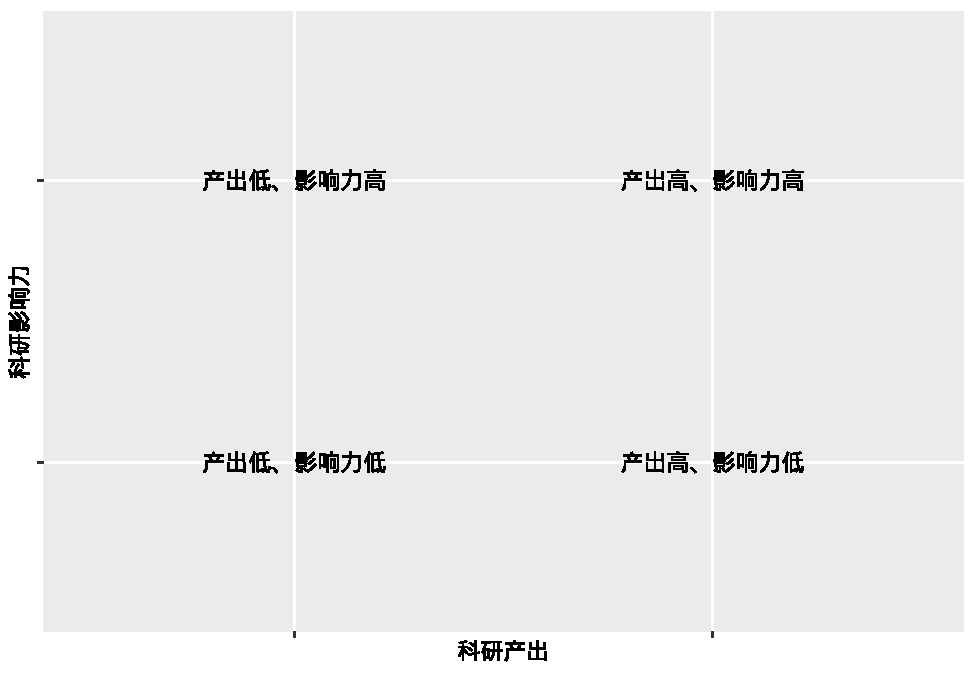
\includegraphics[width=1\linewidth]{ElegantBookdown_files/figure-latex/unnamed-chunk-26-1} \end{center}

看数据呢

\hypertarget{collegecontr}{%
\chapter{学院对学科的贡献}\label{collegecontr}}

本章讨论各学院机构对ESI学科的贡献,由于数据库的不同,统计出来的论文数量和被引频次与ESI数据库存在一定的差异。按照ESI的方法,一篇文章若有多个机构,那么这些机构对学科的贡献是对等的。

\begin{verbatim}
#> [1] "2041-1723"
\end{verbatim}

这篇文章ESI被收录在物理学学科,然而用JCR期刊列表ISSN映射,是交叉学科,这是因为,

\begin{verbatim}
#> # A tibble: 1 x 6
#>   `Full title`          Title29    Title20    ISSN      EISSN `Category name`  
#>   <chr>                 <chr>      <chr>      <chr>     <chr> <chr>            
#> 1 Nature Communications NAT COMMUN NAT COMMUN 2041-1723 null  Multidisciplinary
\end{verbatim}

被归类为跨学科学科(Multidisciplinary field)的Science、Nature与PNAS期刊,会被按照各篇文章的参考文献(reference)与引用文献(citation),重新为每篇文章单独分类,但每篇文章仍只会被分类到一个学科。

\hypertarget{ux5b66ux9662ux5bf9esiux5b66ux79d1ux88abux5f15ux9891ux6b21ux7684ux8d21ux732e}{%
\section{学院对ESI学科被引频次的贡献}\label{ux5b66ux9662ux5bf9esiux5b66ux79d1ux88abux5f15ux9891ux6b21ux7684ux8d21ux732e}}

\begin{center}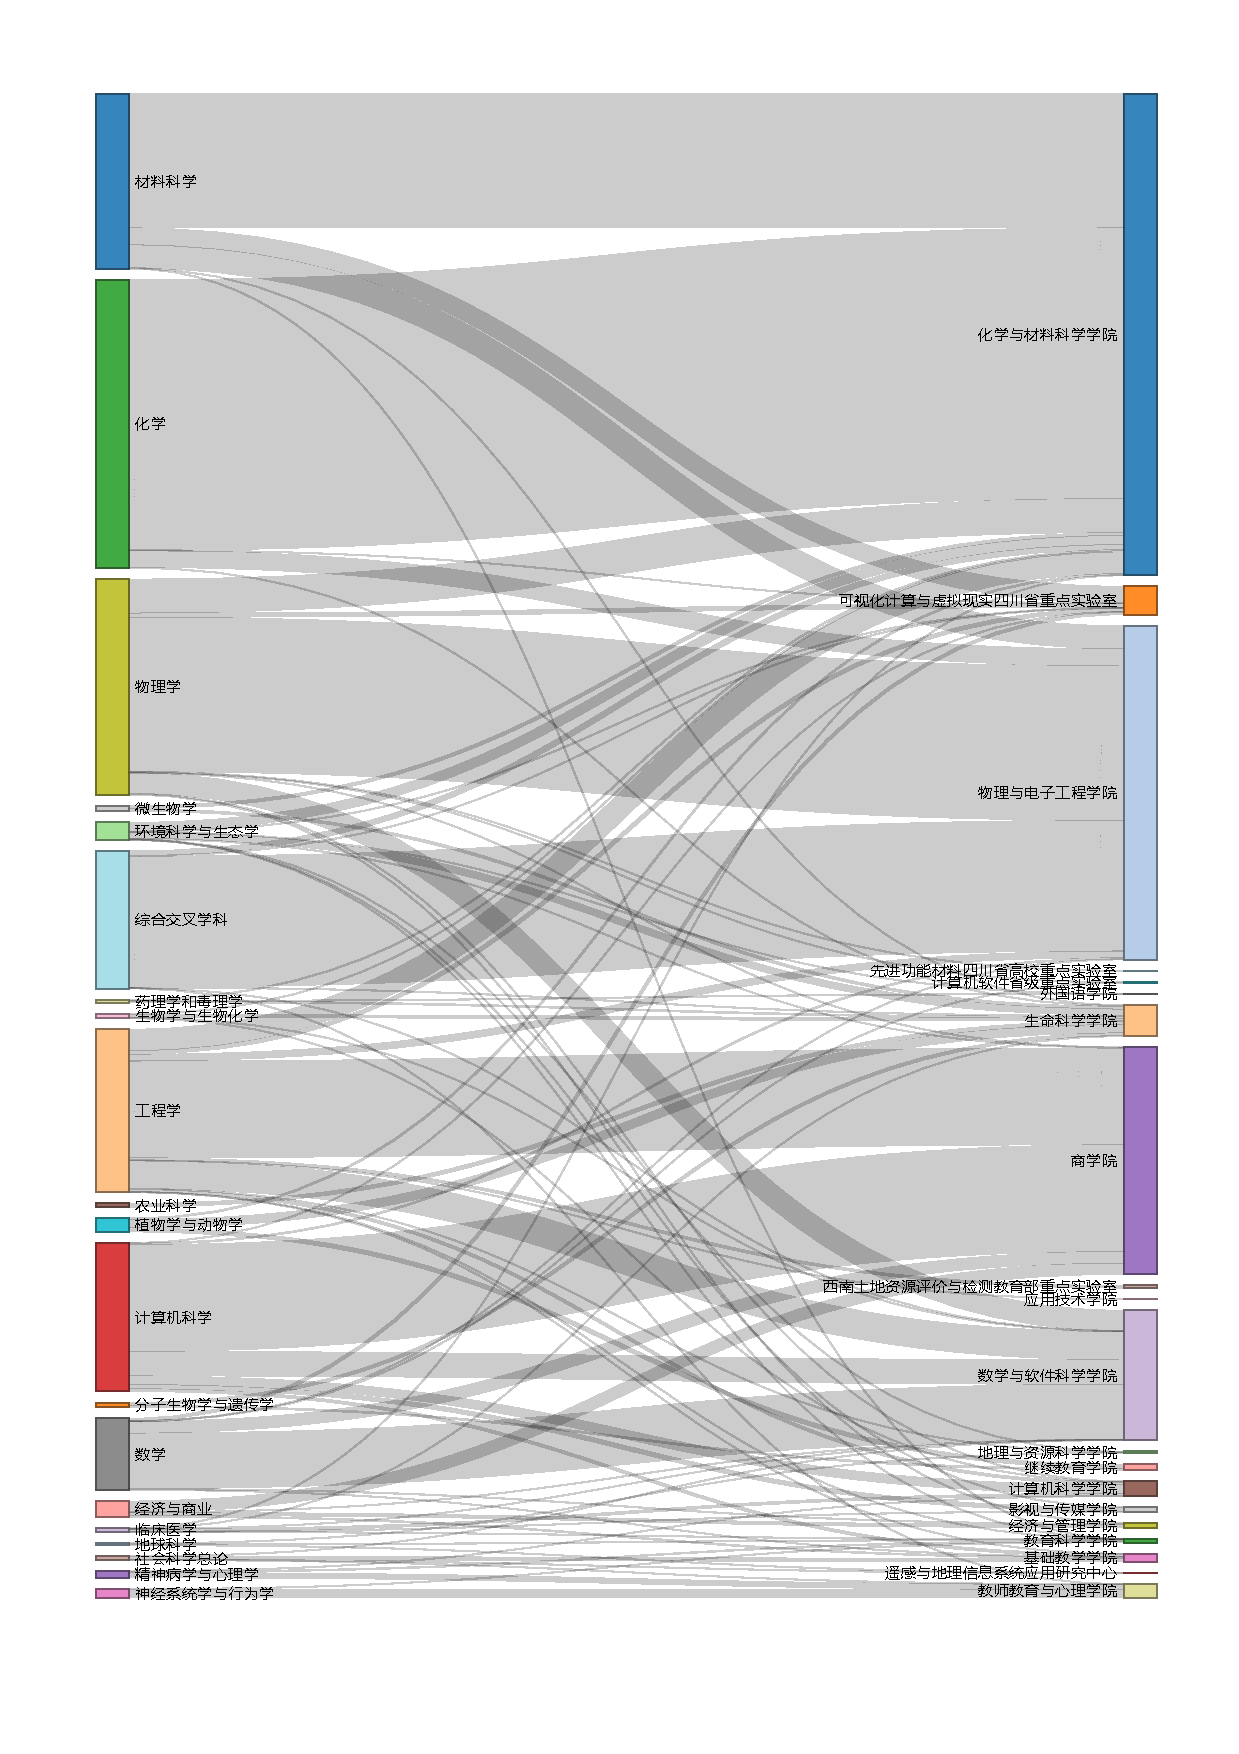
\includegraphics[width=1\linewidth]{sankeyNetwork/sankeyNetwork} \end{center}

具体数据:

因篇幅原因,下面只列出部分学科的情况

另外的方法:

这里我们列出各学院对我校\textbf{工程学学科}学术影响力贡献的具体数据

\begin{table}[!h]

\caption{\label{tab:unnamed-chunk-36}各学院对我校工程学学科学术影响力贡献}
\centering
\begin{tabular}[t]{llrlrl}
\toprule
学科 & 学院 & 论文数 & 论文数占比 & 被引频次 & 被引频次占比\\
\midrule
工程学 & 商学院 & 39 & 19.40\% & 1773 & 59.34\%\\
工程学 & 数学与软件科学学院 & 69 & 34.33\% & 517 & 17.30\%\\
工程学 & 化学与材料科学学院 & 39 & 19.40\% & 393 & 13.15\%\\
工程学 & 物理与电子工程学院 & 22 & 10.95\% & 121 & 4.05\%\\
工程学 & 可视化计算与虚拟现实四川省重点实验室 & 11 & 5.47\% & 67 & 2.24\%\\
\addlinespace
工程学 & 计算机科学学院 & 9 & 4.48\% & 50 & 1.67\%\\
工程学 & 西南土地资源评价与检测教育部重点实验室 & 1 & 0.50\% & 47 & 1.57\%\\
工程学 & 地理与资源科学学院 & 4 & 1.99\% & 8 & 0.27\%\\
工程学 & 基础教学学院 & 3 & 1.49\% & 4 & 0.13\%\\
工程学 & 教育科学学院 & 1 & 0.50\% & 4 & 0.13\%\\
\addlinespace
工程学 & 应用技术学院 & 2 & 1.00\% & 4 & 0.13\%\\
工程学 & 影视与传媒学院 & 1 & 0.50\% & 0 & 0.00\%\\
\bottomrule
\end{tabular}
\end{table}

\hypertarget{ux5b66ux9662ux5728ux5b66ux79d1ux7684ux5206ux914d}{%
\section{学院在学科的分配}\label{ux5b66ux9662ux5728ux5b66ux79d1ux7684ux5206ux914d}}

和学院对学科的贡献不同,这里是以学院分组,看学院输出的文献,都流向了哪些学科?
可能看问题的角度不同,学科处的领导在乎:\textbf{个人服从学院,学院服从学科,学科服从学校}

就是看物理学院有没有全力投入物理学,而是搞了化学?

\begin{table}[!h]

\caption{\label{tab:unnamed-chunk-38}学院科研产出,都流向了哪些学科}
\centering
\begin{tabular}[t]{llrlrl}
\toprule
coll\_name\_cn & discipline\_cn & n\_paper & n\_paper\_percent & n\_cited & n\_cited\_percent\\
\midrule
化学与材料科学学院 & 化学 & 338 & 52.24\% & 4960 & 56.18\%\\
化学与材料科学学院 & 材料科学 & 171 & 26.43\% & 2462 & 27.89\%\\
化学与材料科学学院 & 物理学 & 43 & 6.65\% & 621 & 7.03\%\\
化学与材料科学学院 & 工程学 & 39 & 6.03\% & 393 & 4.45\%\\
化学与材料科学学院 & 环境科学与生态学 & 29 & 4.48\% & 167 & 1.89\%\\
\addlinespace
化学与材料科学学院 & 综合交叉学科 & 6 & 0.93\% & 94 & 1.06\%\\
化学与材料科学学院 & 微生物学 & 9 & 1.39\% & 55 & 0.62\%\\
化学与材料科学学院 & 植物学与动物学 & 1 & 0.15\% & 31 & 0.35\%\\
化学与材料科学学院 & 药理学和毒理学 & 1 & 0.15\% & 24 & 0.27\%\\
化学与材料科学学院 & 生物学与生物化学 & 8 & 1.24\% & 19 & 0.22\%\\
\addlinespace
化学与材料科学学院 & 临床医学 & 2 & 0.31\% & 3 & 0.03\%\\
商学院 & 计算机科学 & 40 & 42.11\% & 1956 & 47.01\%\\
商学院 & 工程学 & 39 & 41.05\% & 1773 & 42.61\%\\
商学院 & 数学 & 3 & 3.16\% & 212 & 5.09\%\\
商学院 & 经济与商业 & 5 & 5.26\% & 208 & 5.00\%\\
\addlinespace
商学院 & 环境科学与生态学 & 4 & 4.21\% & 11 & 0.26\%\\
商学院 & 物理学 & 2 & 2.11\% & 1 & 0.02\%\\
商学院 & 社会科学总论 & 2 & 2.11\% & 0 & 0.00\%\\
物理与电子工程学院 & 物理学 & 414 & 72.50\% & 2831 & 46.27\%\\
物理与电子工程学院 & 综合交叉学科 & 15 & 2.63\% & 2397 & 39.18\%\\
\addlinespace
物理与电子工程学院 & 材料科学 & 46 & 8.06\% & 424 & 6.93\%\\
物理与电子工程学院 & 化学 & 65 & 11.38\% & 310 & 5.07\%\\
物理与电子工程学院 & 工程学 & 22 & 3.85\% & 121 & 1.98\%\\
物理与电子工程学院 & 计算机科学 & 5 & 0.88\% & 30 & 0.49\%\\
物理与电子工程学院 & 数学 & 2 & 0.35\% & 5 & 0.08\%\\
\addlinespace
物理与电子工程学院 & 神经系统学与行为学 & 1 & 0.18\% & 0 & 0.00\%\\
物理与电子工程学院 & 空间科学 & 1 & 0.18\% & 0 & 0.00\%\\
\bottomrule
\end{tabular}
\end{table}

\hypertarget{jcr}{%
\chapter{期刊}\label{jcr}}

\hypertarget{esiux5b66ux79d1ux8ba4ux5b9aux7684ux671fux520a}{%
\section{ESI学科认定的期刊}\label{esiux5b66ux79d1ux8ba4ux5b9aux7684ux671fux520a}}

也就说,你投这些期刊,才是服从学科了

\begin{verbatim}
#> [1] "Full title"    "Title29"       "Title20"       "ISSN"         
#> [5] "EISSN"         "Category name"
\end{verbatim}

比如物理学科,你投这些期刊,在川师的话你会自摸加一番

\begin{table}[!h]

\caption{\label{tab:unnamed-chunk-40}优秀的物理期刊}
\centering
\begin{tabular}[t]{lll}
\toprule
category\_name & full\_title & issn\\
\midrule
Physics & ACOUSTICAL PHYSICS & 1063-7710\\
Physics & Acoustics Australia & 0814-6039\\
Physics & ACS Photonics & 2330-4022\\
Physics & ACTA ACUSTICA UNITED WITH ACUSTICA & 1610-1928\\
Physics & ACTA PHYSICA POLONICA A & 0587-4246\\
\addlinespace
Physics & ACTA PHYSICA POLONICA B & 0587-4254\\
Physics & ACTA PHYSICA SINICA & 1000-3290\\
Physics & ACTA PHYSICA SLOVACA & 0323-0465\\
Physics & Advanced Science & ****-****\\
Physics & Advances In Atomic Molecular and Optical Physics & 1049-250X\\
\addlinespace
Physics & Advances in Chemical Physics & 0065-2385\\
Physics & Advances in Condensed Matter Physics & 1687-8108\\
Physics & Advances in High Energy Physics & 1687-7357\\
Physics & Advances in Mathematical Physics & 1687-9120\\
Physics & Advances in Optics and Photonics & 1943-8206\\
\bottomrule
\end{tabular}
\end{table}

\hypertarget{predict}{%
\chapter{学科预测}\label{predict}}

在前面一章,我们看到我校的潜力学科是工程学科,有望在2020年进入ESI的1\%学科。本章的主要工作是,计算并预测川师工程学科2020年进入ESI前百分之一学科的概率, 以及竞争对手的概率。

\hypertarget{ux7edfux8ba1ux65b9ux6cd5}{%
\section{统计方法}\label{ux7edfux8ba1ux65b9ux6cd5}}

为了更通俗的解释这个模型,可以把机构的被引频次与人跳远距离进行类比。

每个年龄阶段的人跳远的距离,显然不是一个固定的值,是一个分布。比如,

\begin{itemize}
\tightlist
\item
  小学一年级的学生,跳远距离是一个均值为1.0,方差为2 的正态分布;
\item
  小学二年级的学生,跳远距离是一个均值为1.2,方差为3 的正态分布;
\item
  小学三年级的学生,跳远距离是一个均值为1.5,方差为4 的正态分布;
\item
  \ldots{}
\end{itemize}

均值的变化,就是我们模拟的部分,如果营养保证、训练有方,我们认为均值的变化随时间是一个线性关系。学科发展而言,也是类似的,学校就是一个个小学生,不同的是,被引频次不是正态分布,而是服从负二项式分布,随着事物的发展和时间的推移,在每一个阶段它的分布均值和形状会有些不同。同样,我们模拟均值的变化随时间是一个线性关系。

学科的发展与很多方面都有关系,因此建立一个完全正确的预测模型是不可能的。正如英国统计学家George E. P. Box所说 ``All models are wrong, but some are useful.'' 因此我们的模型是错误的,也可能没什么用,但我们依然坚持呈现出来,用图书馆人质朴的方式为我校的发展呐喊助威。

相关研究表明,科研论文被引频次服从负二项分布(具体可见附录),我们建立贝叶斯线性模型,并给定参数的先验概率:

\begin{align*}
y_i & \sim \text{NegBinomial}(\mu_i, \phi) \\
\log(\mu_i) & = \alpha + \gamma_{j[i]} + \beta x_i \\
\alpha & \sim \text{Normal}(0, 100) \\
\beta & \sim \text{Normal}(0, 10)  \\
\gamma & \sim \text{Normal}(0, 2)  \\
\phi & \sim \text{HalfCauchy}(0, 2.5)
\end{align*}

\hypertarget{ux7ed3ux679cux5206ux6790}{%
\section{结果分析}\label{ux7ed3ux679cux5206ux6790}}

根据模型计算,我们预测了工程学科2020年的科研产出量的估计值282,以及50\%的可信赖区间(107, 417),模型评估见附录。

\begin{center}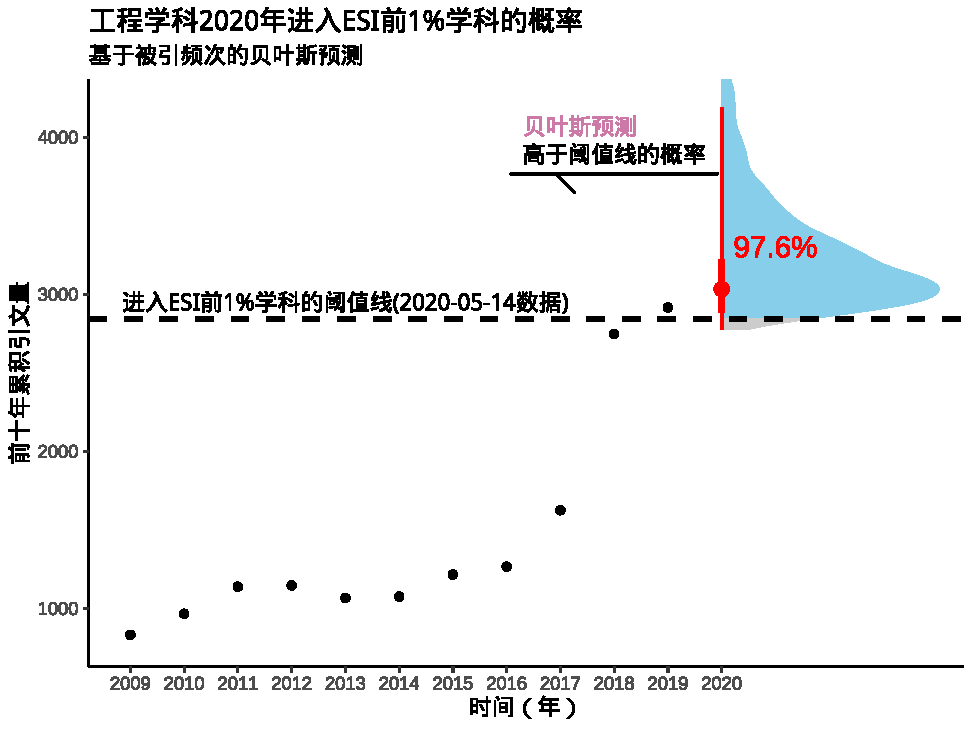
\includegraphics[width=1\linewidth]{ElegantBookdown_files/figure-latex/unnamed-chunk-57-1} \end{center}

因此,四川师范大学近十年的累计科研影响力估计值以及分位数区间见下表\ref{tab:tabestimate} ,在阈值线变化不大或者不变的前提下,2020年进入ESI前百分之一学科的概率将为79.0\%

\begin{table}[!h]

\caption{\label{tab:tabestimate}四川师范大学工程学累计科研影响力估计值以及2020年进入ESI前百分之一学科的概率}
\centering
\begin{tabular}[t]{rrrrl}
\toprule
year\_range & pred\_mean & quantile2.5 & quantile97.5 & prob\_above\_line\\
\midrule
2020 & 3302 & 2845 & 4506 & 97.6\%\\
\bottomrule
\end{tabular}
\end{table}

\begin{center}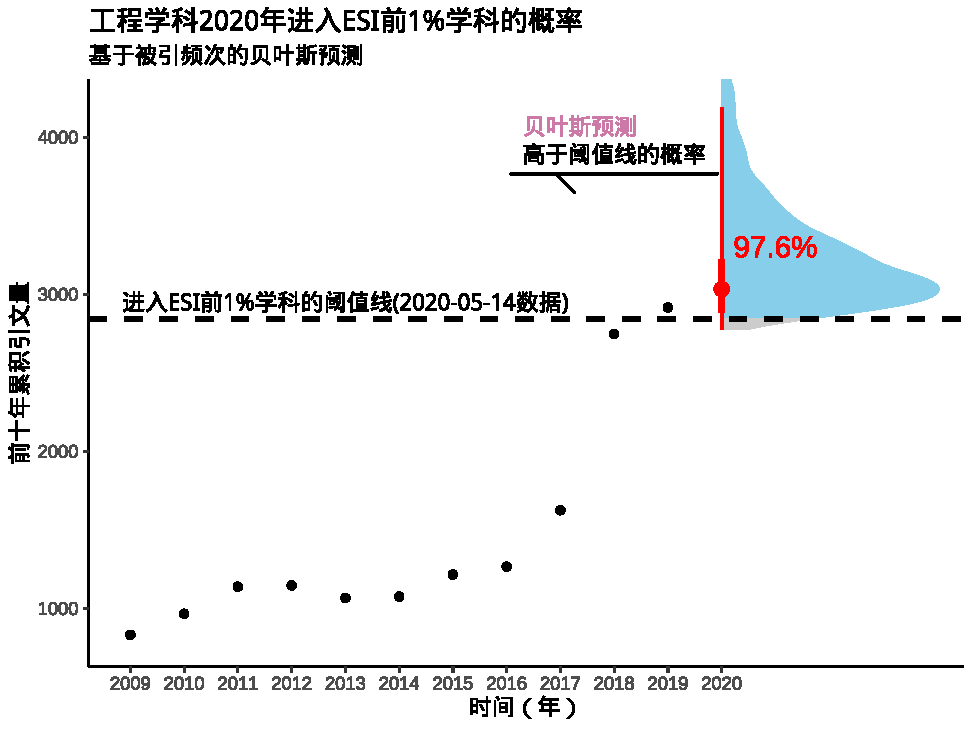
\includegraphics[width=1\linewidth]{ElegantBookdown_files/figure-latex/unnamed-chunk-61-1} \end{center}

\hypertarget{ux7adeux4e89ux5bf9ux624bux7684ux6982ux7387}{%
\section{竞争对手的概率}\label{ux7adeux4e89ux5bf9ux624bux7684ux6982ux7387}}

是否进入ESI前百分之一学科,取决于这个机构近十年累计被引频次,统计的周期是一个滚动的窗口,我们在预测2020年的情况,需要计算2001年-2020年这个时间周期,如果2010年的被引频次很高,而2020年很低,那么十年为窗口的累计量就下滑,因此当前各学校的接近程度高不代表入选的概率也高。这里,我们采用相同的贝叶斯模型,计算竞争对手的工程学科入选概率.

\begin{longtable}[]{@{}lllllll@{}}
\toprule
& univ\_cn & year & pred\_mean & Q2.5 & Q97.5 & prob\_above\_line\tabularnewline
\midrule
\endhead
1 & 广西师范大学 & 2020 & 2694. & 2012 & 5038. & 25.6\%\tabularnewline
2 & 华中师范大学 & 2020 & 3160. & 2543 & 4686. & 68.0\%\tabularnewline
3 & 四川师范大学 & 2020 & 3168. & 2696. & 4269. & 79.3\%\tabularnewline
4 & 重庆师范大学 & 2020 & 2957. & 2638 & 3667. & 60.5\%\tabularnewline
\bottomrule
\end{longtable}

我们是以阈值线不变或者变化很小为前提,进行的预测, 事实上,阈值线每两个月就会调整一次,尽管我们进入ESI学科概率比较大,但也不能掉以轻心。如果需要了解其他学科的预测信息或者对预测模型有不同见解的,非常欢迎与本文作者交流探讨。

\hypertarget{conclusion}{%
\chapter{小结}\label{conclusion}}

在国家``双一流''建设的指导下,师范类高校应把握时机,突出特色,取长补短,积极应对挑战。

\begin{itemize}
\item
  重点抓学科建设,在保持优势学科的基础上,加大对潜力学科的建设力度,进一步优化学科布局,既要增加入围学科数量,还要加强学科内涵建设,实现学科均衡发展。
\item
  改革和完善科研评价体系和考核奖励政策,从目前的根据在SCI、EI、SSCI等权威数据库收录
  的或在学术期刊发表的论文数、专利数、科研成果获奖数、论文引用数等定量指标进行考核和奖励的机制转移到总被引频次、高被引论文数和热门论文数等体现学科内涵的指标上来,更加注重科研创新能力、学术影响力和发展力, 达到科研产量与质量的协同发展,提高科研人员的积极性和创新性。
\item
  加强学术队伍建设,加大高层次人才的引进力度,同时培养具有发展潜力和创新能力的青年骨干,提高科研队伍的整体水平,助力学科产出。
\item
  加强与一流大学和科研机构的实质性合作,促进高校科研人员更加密切地关注国际学术前沿,更快掌握最新、最先进的技术,为开展更具有前瞻性的科学研究提供强大的信息支持和技术保障,从而进一步提升国际影响力和促进``双一流''建设快速发展。
\end{itemize}

\cleardoublepage

\hypertarget{appendix-ux9644ux5f55}{%
\appendix}


\hypertarget{sound}{%
\chapter{贝叶斯模型参数}\label{sound}}

\hypertarget{ux88abux5f15ux9891ux6b21ux4e3aux4ec0ux4e48ux662fux8d1fux4e8cux9879ux5206ux5e03}{%
\section{被引频次为什么是负二项分布}\label{ux88abux5f15ux9891ux6b21ux4e3aux4ec0ux4e48ux662fux8d1fux4e8cux9879ux5206ux5e03}}

\begin{center}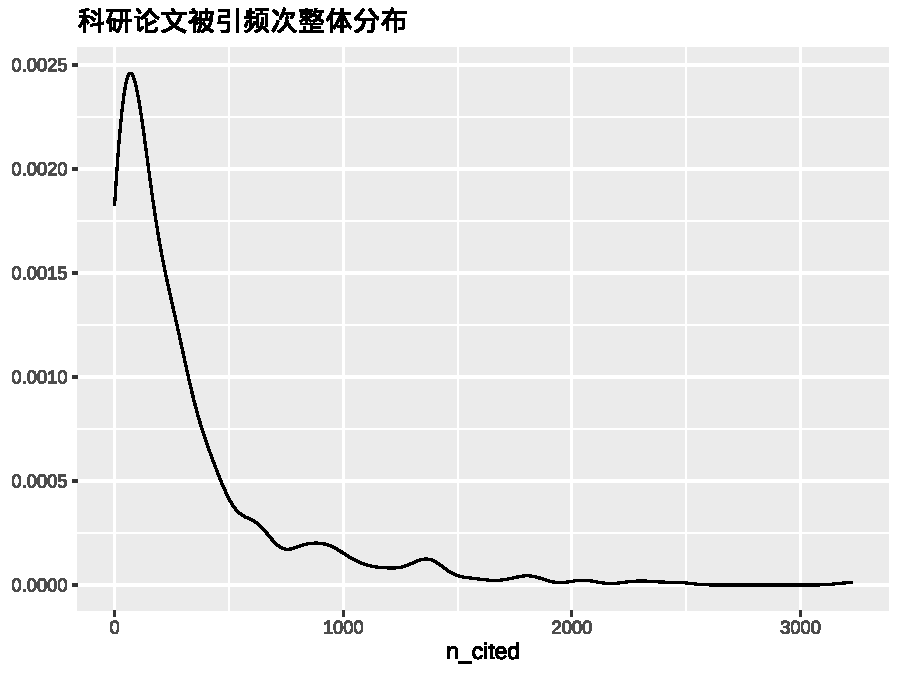
\includegraphics[width=1\linewidth]{ElegantBookdown_files/figure-latex/unnamed-chunk-66-1} \end{center}

\begin{center}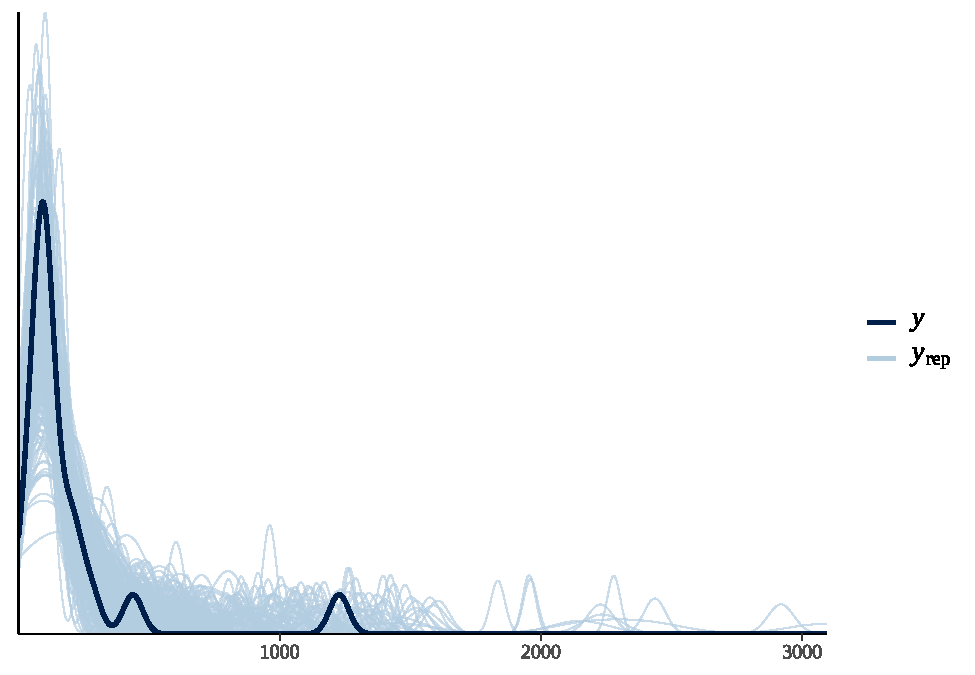
\includegraphics[width=1\linewidth]{ElegantBookdown_files/figure-latex/unnamed-chunk-67-1} \end{center}

\hypertarget{ux540eux9a8cux6982ux7387ux5206ux5e03}{%
\section{后验概率分布}\label{ux540eux9a8cux6982ux7387ux5206ux5e03}}

\begin{center}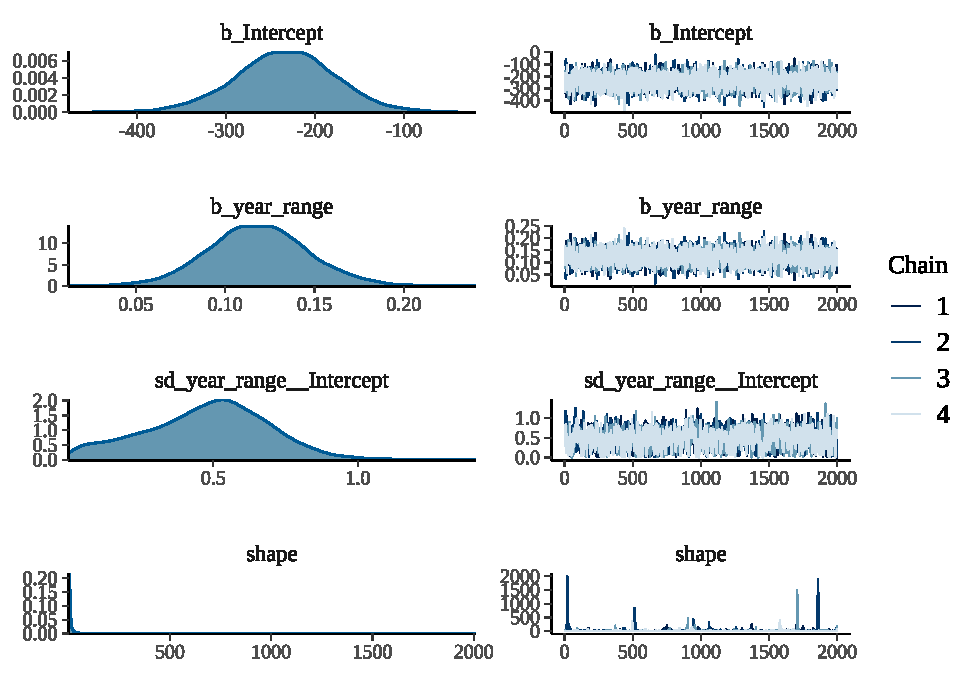
\includegraphics[width=1\linewidth]{ElegantBookdown_files/figure-latex/unnamed-chunk-68-1} \end{center}

\hypertarget{ux540eux9a8cux6982ux7387ux68c0ux9a8c}{%
\section{后验概率检验}\label{ux540eux9a8cux6982ux7387ux68c0ux9a8c}}

\begin{center}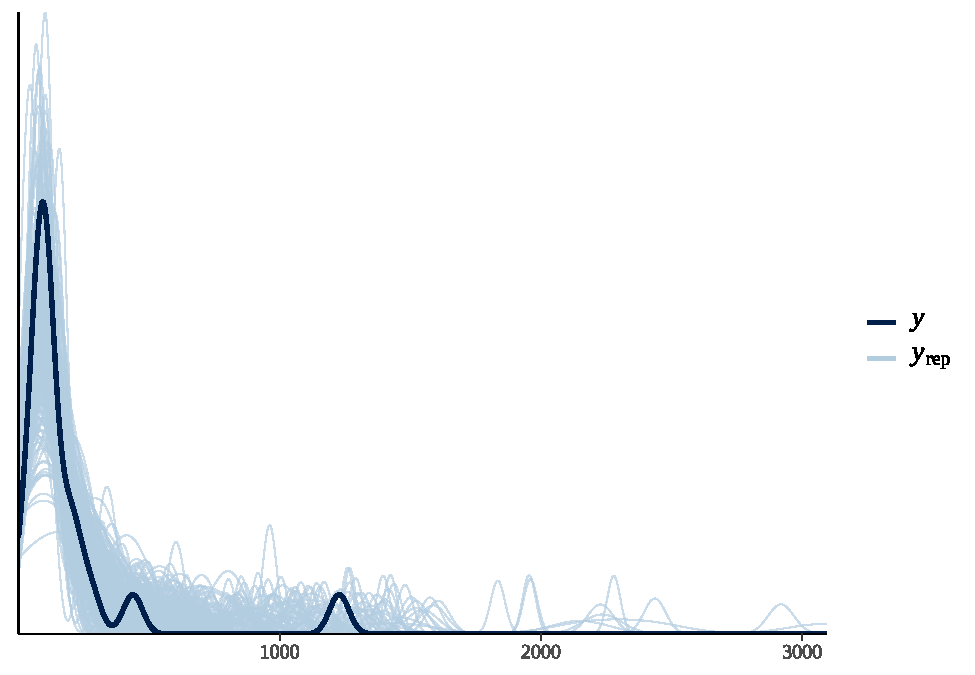
\includegraphics[width=1\linewidth]{ElegantBookdown_files/figure-latex/unnamed-chunk-71-1} \end{center}

\hypertarget{esi-ux6570ux636eux5b8cux5168ux4e0dux900fux660e}{%
\section{ESI 数据完全不透明}\label{esi-ux6570ux636eux5b8cux5168ux4e0dux900fux660e}}

5月14日更新的ESI数据库收录论文的时间范围是2010年------2020年2月底(十年零两个月);

\begin{itemize}
\tightlist
\item
  我们只能检索到出版年。比如,7月份发布时,

  \begin{itemize}
  \tightlist
  \item
    我们能检索的2010年------2020年7月
  \item
    ESI数据库收录论文的时间范围是2010年2月------2020年4月
  \end{itemize}
\item
  在ESI检索到的数据,他们还要再筛查一次。

  \begin{itemize}
  \tightlist
  \item
    ESI工程学和计算机这两个学科的引用有不少是来自会议论文的,但是ESI不统计来自会议论文的引用,所以实际表现没有您检索出的结果那么高。
  \end{itemize}
\item
  学科分类也不能完全一致,尤其是交叉学科的。
\end{itemize}

\hypertarget{References}{%
\chapter*{参考文献}\label{References}}
\addcontentsline{toc}{chapter}{参考文献}

{[}1{]} R Core Team (2013). R: A language and environment for statistical
computing. R Foundation for Statistical Computing, Vienna, Austria.
URL \url{http://www.R-project.org/}.

{[}2{]} Wickham H (2016). ggplot2: Elegant Graphics for Data Analysis. Springer-Verlag New York. ISBN 978-3-319-24277-4

{[}3{]} Wickham, H., Grolemund, G. (2017). R for Data Science: Import, Tidy, Transform, Visualize, and Model Data. O'Reilly Media. ISBN: 1491910399

{[}4{]} Xie Y, Allaire J, Grolemund G (2018). R Markdown: The Definitive Guide. Chapman and Hall/CRC, Boca Raton, Florida. ISBN 9781138359338

{[}5{]} Gelman, A., Lee, D., \& Guo, J. (2015). Stan: A Probabilistic Programming Language for Bayesian Inference and Optimization. Journal of Educational and Behavioral Statistics, 40(5), 530--543.

{[}6{]} Bürkner P (2017). brms: An R Package for Bayesian Multilevel Models Using Stan. Journal of Statistical Software, 80(1), 1--28.

{[}7{]} Kay M (2020). tidybayes: Tidy Data and Geoms for Bayesian Models. doi: 10.5281/zenodo.1308151, R package version 2.0.3

{[}8{]} Andrew Gelman, John Carlin, Hal Stern, David Dunson, Aki Vehtari, and Donald Rubin (2014). Bayesian Data Analysis. 3rd ed.~Chapman and Hall/CRC.

{[}9{]} Kruschke, J. K. (2014). Doing Bayesian data analysis : a tutorial with R and BUGS. Burlington, MA: Academic Press.

{[}10{]} McElreath, R. (2015). \emph{Statistical rethinking: A Bayesian course with examples in R and Stan.} Chapman \& Hall/CRC Press.

{[}11{]} Kruschke, J. K. \& Liddell, T. M. (2018). The Bayesian New Statistics: Hypothesis testing, estimation, meta-analysis, and power analysis from a Bayesian perspective. Psychonomic Bulletin \& Review, 25:178-206.
% 参考文献
\bibliography{book.bib}



% 插入 after_body.tex

\end{document}
